
\section{Anhang}

\subsection{Detaillierter Start des Backends auf dem HIMMUC}\label{par:detailed_himmuc}

Um Mandelbrot manuell auf dem Host-System zu installieren,
müssen zunächst die notwendigen Bibliotheken installiert werden.
Eine Anleitung dazu findet sich in \autoref{par:himmuc_install_libs}.
Dies muss nur einmal ausgeführt werden, anschließend können die
Programme wie in \autoref{par:himmuc_build_backend} beschrieben kompiliert werden.
Ist dies nicht gewünscht oder erledigt muss das Backend lediglich noch wie
in \autoref{par:himmuc_run_backend} beschrieben gestartet werden.


\paragraph{Lokale Installation der Bibliotheken}\label{par:himmuc_install_libs}


Da hierbei davon ausgegangen wird, dass keine root-Rechte auf dem
Server existieren, werden die Bibliotheken hier lokal in \verb|~/.eragp-mandelbrot|
installiert.
Achten Sie darauf, dass sie Schreibrechte auf dem Ordner haben und
falls sie einen anderen Ordner verwenden wollen,
ersetzen sie jedes Vorkommen des Pfades durch ihren Pfad (insbesondere in der Datei \verb|CMakeLists.txt|).
Die MPI-Bibliothek ist auf dem HimMUC Cluster bereits vorinstalliert
und muss daher nicht mehr aufgesetzt werden.
\begin{figure}[h!]
	\begin{lstlisting}[language=bash, caption={Erstellen des Installationsordners}]
mkdir ~/.eragp-mandelbrot
    \end{lstlisting}
\end{figure}

Die 'Header-only' Libraries \verb|websocketpp| und \verb|rapidjson| müssen
lediglich an einen fixen Ort kopiert werden.
Dies erledigen die Befehle aus \autoref{shell:install_header_libs}.

\begin{figure}[h!]
	\begin{lstlisting}[language=bash, caption={Lokale Installation der Bibliotheken \texttt{websocketpp} und \texttt{rapidjson}.}, label={shell:install_header_libs}]
mkdir "~/.eragp-mandelbrot/install"
cd "~/.eragp-mandelbrot/install"
# Installation von websocketpp
git clone --branch 0.7.0 https://github.com/zaphoyd/websocketpp.git websocketpp --depth 1
# Installation von rapidjson
git clone https://github.com/Tencent/rapidjson/
    \end{lstlisting}
\end{figure}


Aus der Bibliothek \verb|boost| muss die Teilbibliothek \verb|boost_system| lokal kompiliert werden
Dazu werden die Befehle aus \autoref{shell:install_boost} ausgeführt,
um die Version 1.67.0 herunterzuladen, zu entpacken und lokal zu installieren.
Beachten Sie, dass das kompilieren auch wie in \autoref{par:himmuc_build_backend} beschrieben
von einem der Boards ausgeführt werden muss.

\begin{figure}[h!]
    \begin{lstlisting}[language=bash, caption={Lokale Installation der Bibliothek boost.}, label={shell:install_boost}]
# Erstellen der notwendigen Ordnerstrukturen
mkdir "~/.eragp-mandelbrot/install"
mkdir "~/.eragp-mandelbrot/local"
# Einrichten des Internetproxys
export http_proxy=proxy.in.tum.de:8080
export https_proxy=proxy.in.tum.de:8080
# Herunterladen und kompilieren der Boost-Bibliothek
cd "~/.eragp-mandelbrot/install"
wget "https://dl.bintray.com/boostorg/release/1.67.0/source/boost_1_67_0.tar.bz2"
tar --bzip2 -xf boost_1_67_0.tar.bz2
cd boost_1_67_0
./bootstrap.sh --prefix="$HOME/.eragp-mandelbrot/local/" --with-libraries=system
./b2 install
    \end{lstlisting}
\end{figure}

\paragraph{Kompilieren des Backends}\label{par:himmuc_build_backend}

Stellen Sie zunächst sicher, dass auf dem Cluster die Quelldateien des Backendes (im Ordner \verb|backend/|) liegen
(zum Beispiel über \verb|rsync| oder indem sie das Repository dort auch klonen)
Zum Kompilieren des Backends sollte sich auf einen Raspberry Pi oder ODroid
per ssh eingeloggt werden\footnote{Es existiert ein Entwicklerzugang zu einem geteilten Raspberry Pi über die Adresse \url{sshgate-gepasp.in.tum.de}. Dieser wird auch vom Pythonskript genutzt}

Auf dem Board, aus dem Ordner des Backendquellcodes müssen Sie zum kompilieren
des Backendes die Befehle aus \autoref{shell:himmuc_compile_backend} ausführen.

\begin{figure}[h!]
	\begin{lstlisting}[language=bash, caption={Kompilieren des Backends}, label={shell:himmuc_compile_backend}]
# Erstellen und betreten eines build Ordners
mkdir build
cd build
# Aktivieren der MPI Bibliothek
module load mpi
# Kompilieren
cmake ..
make
    \end{lstlisting}
\end{figure}


\paragraph{Ausführen des Backends}\label{par:himmuc_run_backend}

Um das Backend auf dem HimMUC Cluster laufen zu lassen, muss sich zunächst darauf per ssh eingeloggt werden.
Damit für das Frontend kein Unterschied dazwischen besteht, ob das Backend im Dockercontainer , oder
auf einem externen Server ausgeführt wird, ist bei der ssh-Verbindung der Port 9002
des \verb|himmuc.caps.in.tum.de|-Servers an den lokalen Port 9002 gebunden.
So ist das Backend stets unter \url{localhost:9002} verfügbar.
Der zugehörige Befehl zum Login lautet demnach:

\begin{lstlisting}[language=bash]
ssh <rechnerkennung>@himmuc.caps.in.tum.de -L localhost:9002:localhost:9002
\end{lstlisting}

Anschließend muss aus dem Ordner, in dem die ausführbaren Dateien liegen,
für gewöhnlich also der \verb|~/.eragp-mandelbrot/build/| Ordner,
folgender Befehl ausgeführt werden:

\begin{lstlisting}[language=bash]
srun -p <odr|rpi> -n <number of workers+1> -N <number of nodes/raspis> -l --multi-prog <path to eragp-mandelbrot/backend>/himmuc/run.conf &
ssh -L 0.0.0.0:9002:localhost:9002 -fN -M -S .tunnel.ssh <odr|rpi><host number>
\end{lstlisting}

Dabei bestimmt \verb|-n| die Anzahl der laufenden Prozesse (Also Hostprozess und Workerprozesse)
und \verb|-N| die Anzahl zu verwendender Rechenknoten.
Damit anschließend noch alle Anfragen an den Websocketserver auf dem Hostknoten weitergeleitet werden,
muss noch der Port 9002 des \url{himmuc.in.caps.tum.de}-Servers an den Port 9002 des Rechenknotens gebunden werden,
auf dem der Hostprozess läuft.
Der korrekte Knoten ist dabei der Ausgabe des \verb|srun|-Befehles zu entnehmen.
Eine beispielhafte Ausgabe ist in \autoref{shell:himmuc_running_backend_example} zu sehen.

\begin{figure}[h]
	\begin{lstlisting}[language=bash, caption={Beispielhafter Start des Backends. Hierbei ist der Knoten des Hostprozesses \texttt{rpi03}.}, label={shell:himmuc_running_backend_example}]
muendler@vmschulz8:~/eragp-mandelbrot/backend/build$ srun -N4 -n5 -l --multi-prog ../himmuc/run.conf
srun: error: Could not find executable worker
4: Worker: 4 of 5 on node rpi06
2: Worker: 2 of 5 on node rpi04
3: Worker: 3 of 5 on node rpi05
0: Host: 0 of 5 on node rpi03
0: Host init 5
1: Worker: 1 of 5 on node rpi03
0: Core 1 ready!
1: Worker 1 is ready to receive Data.
2: Worker 2 is ready to receive Data.
0: Listening for connections on to websocket server on 9002
0: Core 2 ready!
3: Worker 3 is ready to receive Data.
0: Core 3 ready!
4: Worker 4 is ready to receive Data.
0: Core 4 ready!
muendler@vmschulz8:~/eragp-mandelbrot/backend/build$ ssh ssh -L 0.0.0.0:9002:localhost:9002 -fN -M -S .tunnel.ssh rpi03
    \end{lstlisting}
\end{figure}

\paragraph{Stoppen des Backends}

Um das Backend wieder zu stoppen, müssen der ssh-Tunnel zur Verbindung der Ports
und der \verb|srun|-Prozess gestoppt werden.
Letzterer lässt sich nach dem dämonisieren im vorigen Aufruf nur über die Prozess-ID finden.
Diese zeigt das Tool \verb|ps| an.
\begin{lstlisting}[language=bash]
ssh -S .tunnel.ssh -O exit rpi<host number>
# To stop the node allocation
scancel -u <user name>
\end{lstlisting}

\subsection{Detaillierte Beschreibung der Header und der CMake Instruktionen}

Die zusammenstellung der ausführbaren Dateien wird in CMake definiert.
Dabei unterscheiden sich diese lediglich in den eingebundenen Quelldateien:
In die Datei \verb|host| werden \verb|host.main.cpp| und \verb|actors/Host.cpp| eingebunden, während
in \verb|worker| \verb|worker.main.cpp| und \verb|actors/Worker.cpp| eingebunden werden.

Diese und alle weiteren Build-Vorgaben werden in der Datei \verb|CMakeLists.txt| für
\verb|cmake|\footnote{Ein Programm, welches die Erstellung von Makefiles vereinfacht in dem es sie automatisch an die Umgebung des Build-Systems anpasst. \url{https://cmake.org/}}
in der hier beschriebenen Reihenfolge spezifiziert.
Es sollte hierbei eine CMake-Version über 3.7.0 gewählt werden und die C++11 Standards\footnote{\url{https://isocpp.org/wiki/faq/cpp11}} werden vorrausgesetzt.
Zudem werden für das Projekt "Mandelbrot" werden alle Dateien im Order \verb|include| eingebunden.
In diesem Ordner liegen die Header-Dateien für alle projektinternen C++-Quelldateien.
Anschließend werden alle C++-Quelldateien (Endung "\verb|.cpp|") aus dem Ordner \verb|src| in einer Liste gesammelt, mit Ausnahme jedoch der oben genannten, exklusiven Quelldateien.
Die erzeugte Liste und die jeweils exklusiven Dateien werden dann den ausführbaren Dateien \verb|host| und \verb|worker| zugeordnet.

Um die verwendeten Bibliotheken verfügbar zu machen werden anschließend die Header der installierten MPI-Bibliothek
sowie die Header der Bibliotheken rapidjson\footnote{\url{http://rapidjson.org}}, websocketpp\footnote{\url{https://github.com/zaphoyd/websocketpp}} und boost\footnote{\url{https://www.boost.org/}}
Diese werden respektive verwendet um JSON zu parsen und enkodieren, Websocket-Verbindungen aufzubauen und darüber zu kommunizieren sowie um diese Bibliothek zu unterstützen.
Da für die boost Bibliothek dabei Header nicht genügen und die systemweite Verfügbarkeit der kompilierten boost-Bibliothek nicht garantiert werden kann, wird die Teilbibliothek boost\_system statisch
in die ausführbaren Datei \verb|host| eingebunden.

Zuletzt werden über Compilerflags alle Kompilierfehler und -warnungen aktiviert sowie die POSIX-Thread-Bibliothek eingebunden,
die Optimierung auf die höchste Stufe gesetzt und spezielle Flags für die Websocketlibrary und MPI gesetzt.

\subsection{Beispielhafte Einbindung der MPI-Initialisierungsfunktion}

Ein beispielhafter Aufruf der Prozessinitialisierung von einer Mainfunktion aus ist in \autoref{src:host.main.cpp} zu sehen. Damit wird MPI initialisiert und nach der
erfolgreichen Initialisierung der eigentliche \hyperref[cls:Host]{Host-Prozess} über \verb|Host::init| gestartet.

\begin{figure}[h]
	\lstinputlisting[caption={Initialisierung des Host-Prozesses in host.main.cpp}, label={src:host.main.cpp}]{../../backend/src/host.main.cpp}
\end{figure}

\begin{figure}
	\lstinputlisting[caption={Initialisierung der MPI-Prozesse in init.cpp}, label={src:init.cpp}, firstline=15, lastline=39, firstnumber=15]{../../backend/src/init.cpp}
\end{figure}

\subsection{Detaillierter Ablauf der Host::handle\_region\_request Methode}

Nach dem Parsen der Nachricht wird die Region global festgelegt und beim korrekten Lastbalancierer eine Zerlegung der angefragten Region über \verb|Balancer::balanceLoad| gestartet.

Jeder Region wird ein Worker zugewiesen.
Dabei ist der Rang des Workers, der eine Region berechnen soll genau der Index der Region in dem zurückgegebenen Array.
Ist ein Worker nicht verfügbar, so werden sein und alle folgenden Ränge um eins erhöht (siehe \autoref{src:Host.cpp.handle_region_request}).
Damit kann der Websocketprozess unabhängig von der tatsächlichen Verteilung den Rang des berechnenden Worker-Prozesses
bestimmen und in der Antwort an den Client zu der Aufteilung der Prozesse einfügen.
Die Struktur und eine gültige Antwort des Websocketservers kann \autoref{src:region.json} entnommen werden.

Nachdem die Aufteilung als Antwort auf die Anfrage dem Websocketprozess bereitgestellt wurde, werden die Teilregionen in eine per Mutexlock-gesicherte Datenstruktur
gelegt. Der MPI verwendende Thread, der diese Regionen anschließend an die Worker sendet wird über das Setzen des booleschen Wertes \verb|mpi_set_regions|
auf \verb|true| darüber informiert, dass neue Regionen zum versenden zur Verfügung stehen.

Indem die Regionaufteilung zuerst an das Frontend und anschließend an die Worker gesendet wird,
wird sichergestellt, dass das Frontend alle empfangenen Regionsdaten korrekt der angefragten Region zuordnen kann.
Dabei wird zwar Rechenzeit verschenkt, jedoch steigt durch die Erstellung sehr kleiner oder leerer Teilregionen
die Wahrscheinlichkeit, dass ein Arbeiter mit seiner Region zu früh abgeschlossen ist.
Würde dann dessen Region vor der Gesamtaufteilung beim Frontend ankommen, besteht die Gefahr,
dass es die Daten verwirft.

\begin{figure}
	\lstinputlisting[caption={Algorithmus zur Zuordnung von Regionen auf Worker in Host.cpp}, label={src:Host.cpp.handle_region_request}, firstline=222, firstnumber=222, lastline=231]{../../backend/src/actors/Host.cpp}
\end{figure}

\begin{figure}
	\lstinputlisting[caption={Ausschnitt aus einer gültigen Antwort auf die Region aus \autoref{src:regionRequest.json} in JSON}, label={src:region.json}, language=json]{./code/region.json}
\end{figure}

\subsection{Beispiele für versendete Daten}

\begin{figure}[!h]
	\lstinputlisting[caption={Ausschnitt aus den Daten einer versendeten Teilregion. Punkt (x,y) liegt in \texttt{"data"} an Index $i=x+y*width$.}, label={src:regionData.json}, language=json]{./code/regionData.short.json}
\end{figure}

\subsection{Nutzbarkeit einzelner Worker}

Es besteht die Möglichkeit, explizit zu definieren ob ein Worker Rechenaufträge bekommen soll oder nicht.
Hierzu existiert im Host das globale Boolean-Array usable\_nodes.
Ein Prozess mit Rang x ist benutzbar, wenn usable\_nodes am Index x true ist.
Nicht benutzbar ist er, wenn die Variable auf false gesetzt ist.
Zudem existiert noch die globale Variable usable\_nodes\_count, die angibt wie viele Worker benutzbar sind.
Genutzt wird dieses Feature, falls beim \hyperref[para:init_worker_test]{Initialen Test aller Worker} Worker als nicht benutzbar eingestuft werden.
%TODO: Eventuell noch anmerken, dass man in einer zukünftigen Version herausfinden könnte, ob Worker nach ihrem initialen Test absturzen. Dann kann man sie gleich auf diese Weise ausschalten.

\paragraph{Initialer Test aller Worker}\label{para:init_worker_test}

Bevor Rechenaufträge an die Worker weitergeleitet werden, wird zunächst jeder Worker einzeln getestet.
Dies dient auch dazu, den Workern den Rang des Hosts zu übermitteln.

Dazu sendet der Host mittels der nicht-blockierenden, synchronen Sendeoperation MPI\_Issend einen Test-Wert an alle Worker.
Durch die synchrone Eigenschaft wird die Operation erst abgeschlossen, wenn eine passende Empfangsoperation gestartet und der Sendeoperation zugeordnet wurde.
Es wurde eine nicht-blockierende Sendeoperation gewählt, um den Test für alle Worker parallel ausführen zu können.

Wurden alle Sendeoperationen gestartet, muss auf deren Abschluss gewartet werden.
Falls nun ein Worker nicht wie erwartet reagiert und die Empfangsoperation nicht durchführt, muss das Warten auf den Abschluss der Sendeoperation abgebrochen werden können.
Deshalb wird MPI\_Testsome in einer Endlosschleife genutzt, die nur abbricht falls alle Sendeoperationen erfolgreich waren (alle MPI\_Requests sind MPI\_REQUEST\_NULL, wodurch MPI\_Testsome in outcount MPI\_UNDEFINED zurückgibt) oder ein Timer abgelaufen ist.
Falls eine oder mehrere Sendeoperationen innerhalb eines Schleifendurchlaufs erfolgreich abgeschlossen wurden, wird deren MPI\_Request auf MPI\_REQUEST\_NULL gesetzt um dies explizit zu zeigen.
Sie werden in den nächsten Schleifendurchläufen von MPI\_Testsome ignoriert.

Nachdem die Schleife abgebrochen wurde, muss noch überprüft werden, welche Sendeoperationen erfolgreich waren und welche nicht.
War die Operation erfolgreich, wird der entsprechende Worker als nutzbar eingestuft.
Falls nicht, wird die noch laufende Sendeoperation mit MPI\_Cancel abgebrochen und der Worker als nicht benutzbar eingestuft.

\subsection{Entwicklung des Beschleunigungsfaktors von SIMD für höhere Iterationszahlen}
\label{par:SIMD-speedup-entwicklung}

Wie durch den konstanten Mehraufwand der SIMD-Verwendung zu erwarten, steigt der Beschleunigungsfaktor
monoton und wächst ab circa 6000 Iterationen pro Pixel nicht mehr wesentlich.
Dies kann \autoref{fig:SIMD-speedup-vs-comptime-10000} entnommen werden.

\begin{figure}
	\centering
	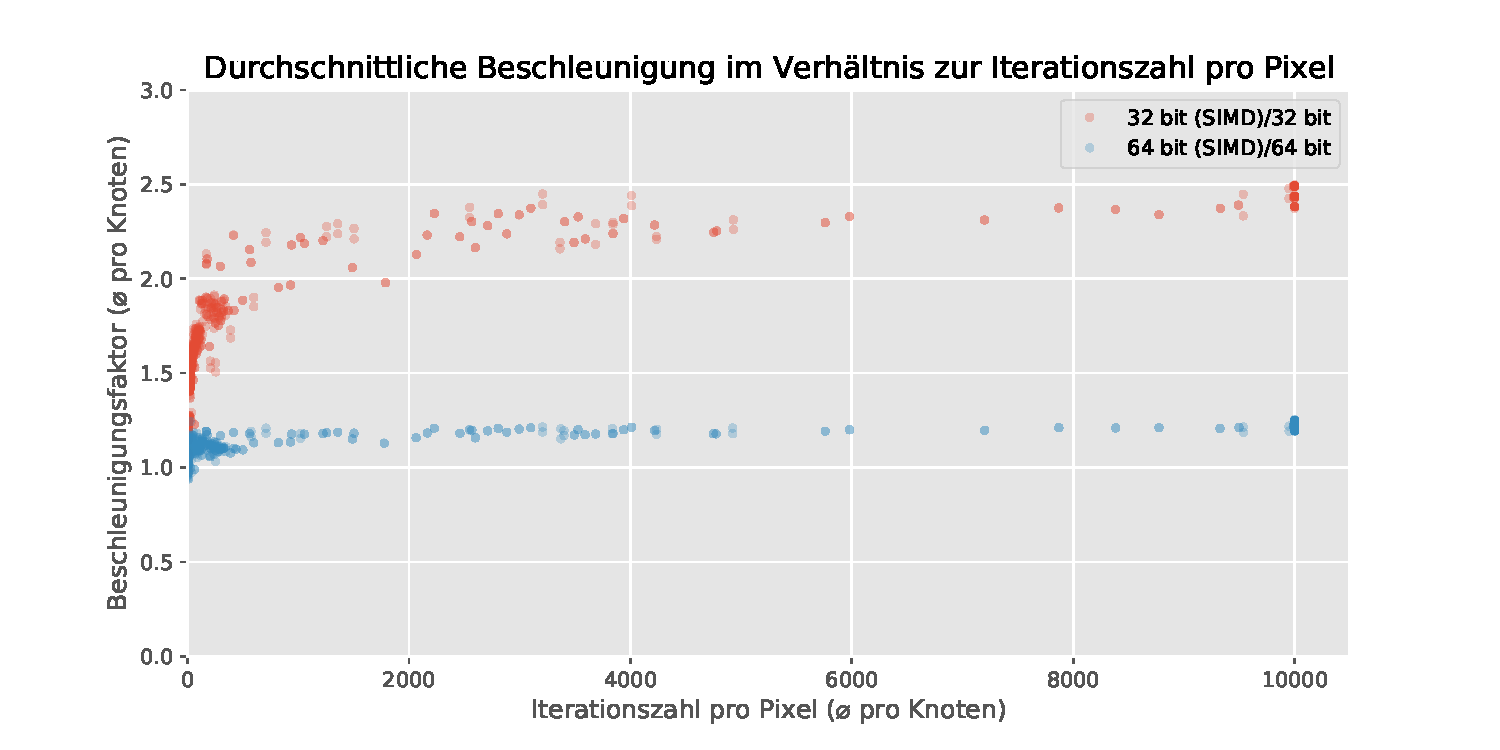
\includegraphics[width=0.9\linewidth]{img/Evaluation/simd/speedup10000.pdf}
	\caption{Beschleunigungsfaktor durch SIMD in Abhängigkeit von der durchschnittlichen Iterationszahl. Auswertung von 360 Regionen mit zwei Durchläufen. Die Iterationszahl für einen Abbruch war 10000.}
	\label{fig:SIMD-speedup-vs-comptime-10000}
\end{figure}

Dass hier auch nicht in der Homogeninät der Iterationszahlen in Bereichen hoher Rechenintensität liegt,
zeigt \autoref{fig:SIMD-speedup-vs-comptime-150}.
Sie hat jedoch einen deutlich erkennbaren Einfluss auf die Beschleunigung.
Während in bei einem frühzeitigen Abbruch bei \hyperref[fig:SIMD-speedup-vs-comptime]{1019 Iterationen} eine Beschleunigung von über 2
erst ab etwa 200 Iterationen gemessen wird, tritt sie bei \hyperref[fig:SIMD-speedup-vs-comptime-150]{maximal 150 Iterationen} bereits ab etwa 140 auf.

\begin{figure}
	\centering
	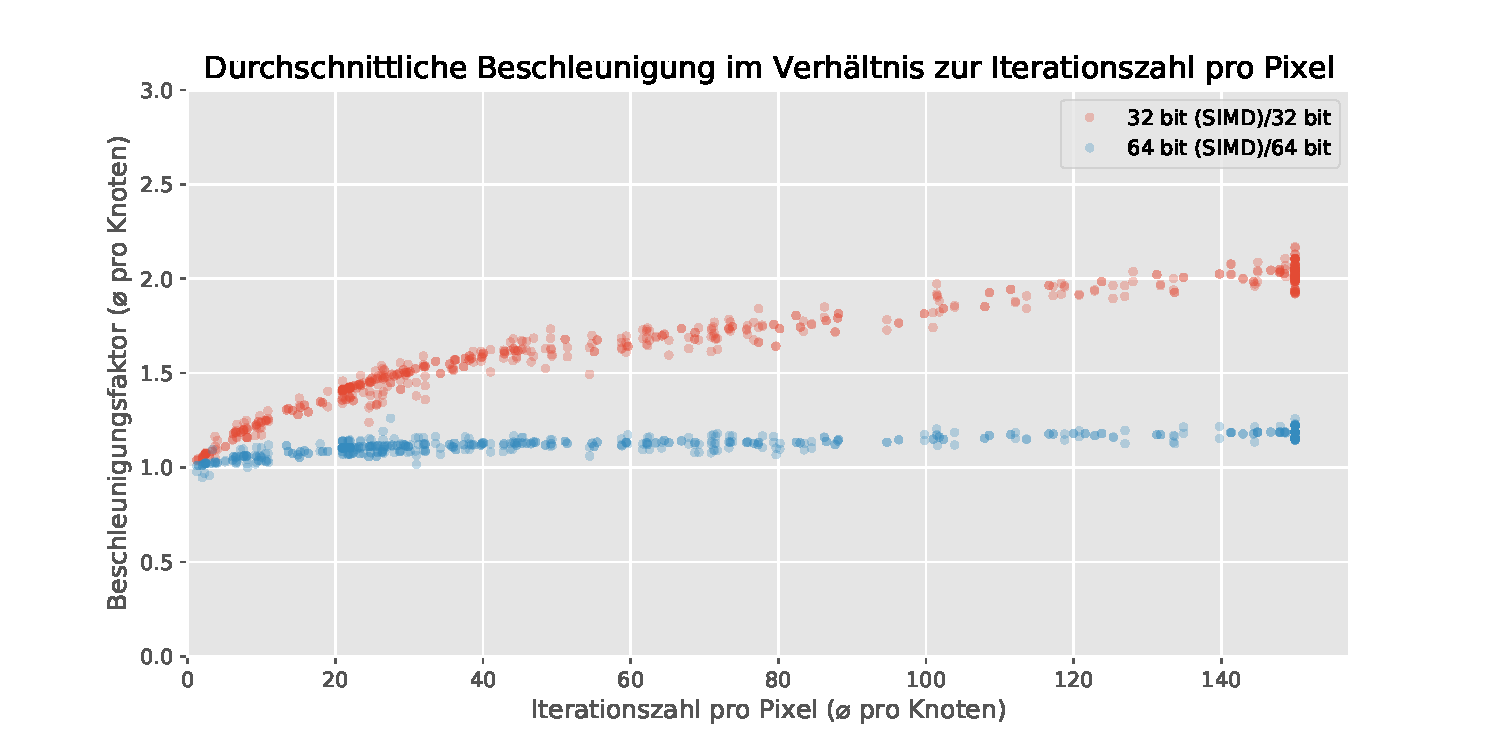
\includegraphics[width=0.9\linewidth]{img/Evaluation/simd/speedup150.pdf}
	\caption{Beschleunigungsfaktor durch SIMD in Abhängigkeit von der durchschnittlichen Iterationszahl. Auswertung von 360 Regionen mit zwei Durchläufen. Die Iterationszahl für einen Abbruch war 150.}
	\label{fig:SIMD-speedup-vs-comptime-150}
\end{figure}